\apendice{Especificación de diseño}

\section{Introducción}

El apéndice de especificación de diseño tiene como objetivo presentar al lector los aspectos del proyecto relativos al diseño de datos, el diseño procedimental y el diseño arquitectónico empleados en la aplicación.

El apartado de \hyperref[sec:datadesign]{diseño de datos} tiene como objetivo señalar el diseño de las entidades utilizado para el almacenamiento de la información manejada por la aplicación. La sección del \hyperref[sec:proceduraldesign]{diseño procedimental} introduce los flujos de interacción del usuario con la aplicación y entre sus componentes para la realización de las acciones planteadas en el apartado de requisitos funcionales. Finalmente el capítulo de \hyperref[sec:archdesign]{diseño arquitectónico} presenta la estructuración de los diversos componentes de la aplicación de acuerdo con el uso de una arquitectura de microservicios.

\section{Diseño de datos} \label{sec:datadesign}

El diseño de datos de la aplicación se ha diseñado a través del uso del ORM (Object–Relational Mapping) para Python SQLAlchemy conectado la aplicación con una base de datos de MariaDB. La utilización de un ORM facilita la interacción de los componentes de la aplicación con la base de datos, permitiendo interactuar con los datos de manera sencilla a través de objetos que actúan como intermediarios en el intercambios de la información.

En el diagrama relacional que se presenta a continuación (véase \autoref{fig:er_diagram}), se pueden observar las relaciones entre las entidades utilizadas por la aplicación, así como los atributos que estas entidades manejan. 

Las entidades ''Repositorio'', ''Incidencia'' y ''Comentario'' representan la manera en la que la información extraída desde GitHub por la aplicación es almacenada en la base de datos. Los repositorios almacenan el nombre, descripción y etiquetas que estos poseen. Los repositorios pueden mantener múltiples incidencias de las cuales se almacena su autor, título, descripción, etiquetas y un parámetro que nos indica si esa incidencia se corresponde con una petición de incorporación de cambios o no. A su vez, las incidencias pueden disponer de comentarios de los cuales se almacena su autor y la información del propio comentario.

\begin{figure}[!ht]
	\centering
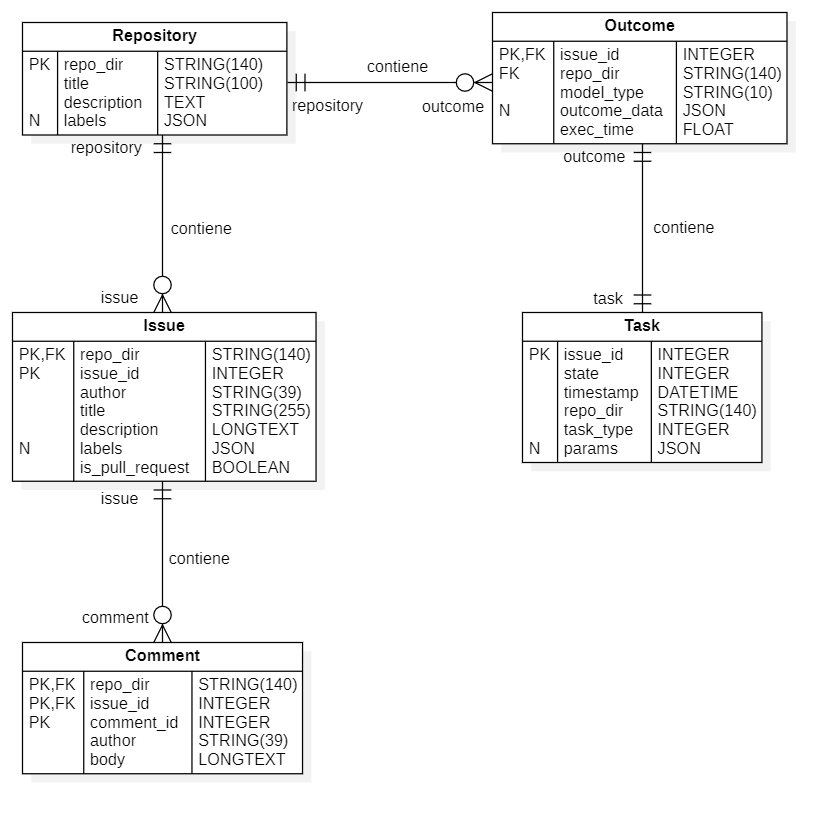
\includegraphics[width=\textwidth]{img/er_diagram.png}
	\caption{Esquema relacional de la base de datos.}
	\label{fig:er_diagram}
\end{figure}

La entidad ''Tarea'' representa la manera en la que se ha decidido generar la interacción entre los componentes del sistema. Con el objetivo de manejar y mantener un registro de las acciones llevadas a cabo por la aplicación se recurrió al uso de entidades ''Tarea'' para establecer una comunicación entre los componentes de la aplicación. Los servicios que componen la aplicación mantienen un proceso que consulta la base de datos de manera periódica en busca de tareas que concuerden con su objetivo y se mantengan en un estado a la espera de ser procesadas.

Finalmente, se puede observar una entidad ''Salida'' que representa los resultados de los experimentos lanzados. Mediante esta entidad se almacenan los resultados obtenidos posteriormente a la aplicación de los modelos de procesamiento del lenguaje natural, así como el tipo de modelo aplicado y el tiempo de ejecución que ha sido requerido para la obtención del resultado. Las salidas se relacionan con el repositorio cuyos datos han sido empleados para la aplicación del modelo.

\section{Diseño procedimental} \label{sec:proceduraldesign}

El diseño procedimental de la aplicación se presenta en el siguiente apartado a partir de los principales flujos de actividad que se desencadenan entre los componentes de la aplicación al lanzar las peticiones contra la API REST.

Podemos distinguir dos actividades fundamentales en la aplicación, las cuales son: la obtención de la información de los repositorios a partir de GitHub (véase \autoref{fig:sec_diagram_extract_repo}), y el lanzamiento de experimentos contra los datos extraídos de los repositorios (véase \autoref{fig:sec_diagram_run_experiment}). Ambos procesos se presentan en los siguientes diagramas de actividad. 

La comunicación entre procesos viene dada mediante dos tipos de relaciones: síncronas, representadas mediante flechas cuyo extremo se encuentra relleno, y asíncronas, representadas por flechas cuyo extremo solo se encuentra delineado. En cuanto a los recuadros de alternancia, representan los flujos de actividad alternativos producidos en función del resultado obtenido por la realización de una llamada.

\begin{sidewaysfigure}[!ht]
	\centering
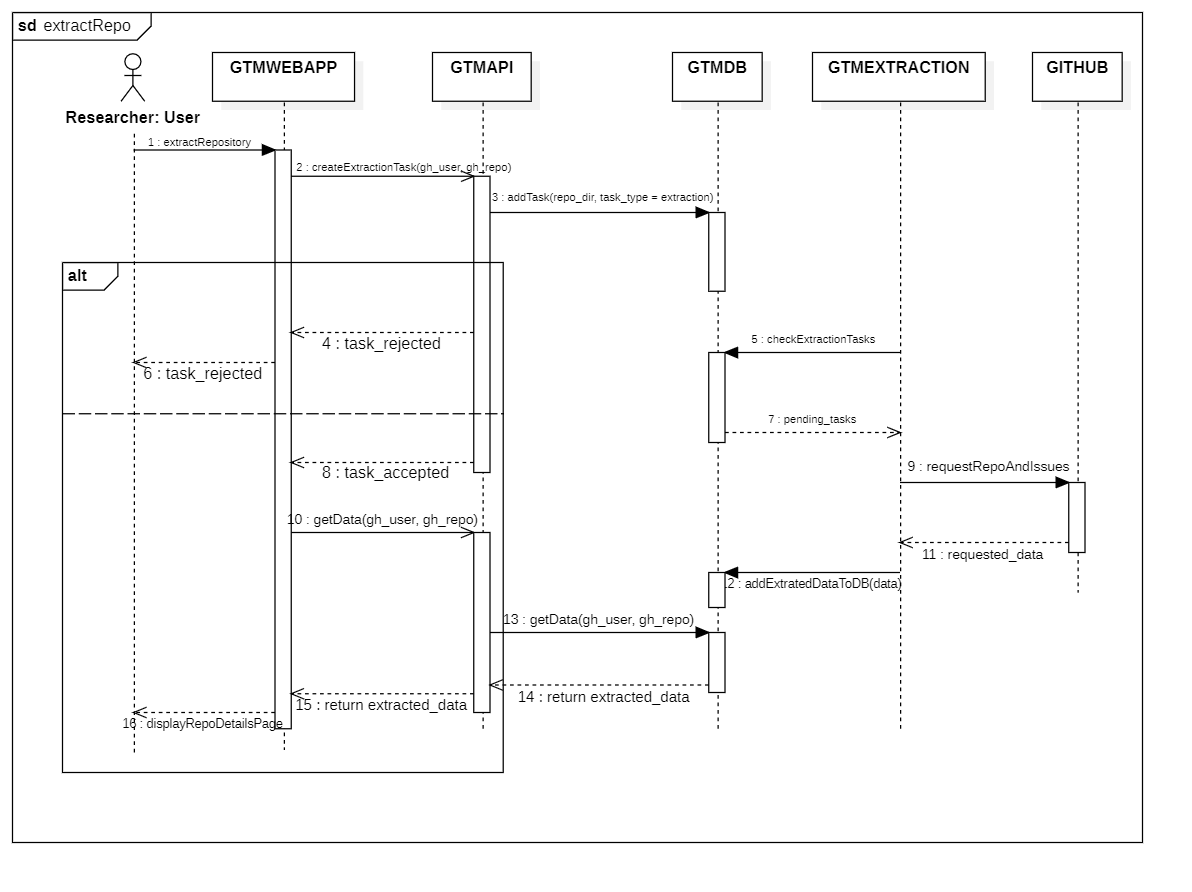
\includegraphics[width=\textwidth]{img/sec_diagram_extract_repo.png}
	\caption{Diagrama de secuencia correspondiente a la extracción de los datos de un repositorio.}
	\label{fig:sec_diagram_extract_repo}
\end{sidewaysfigure}

\begin{sidewaysfigure}[!ht]
	\centering
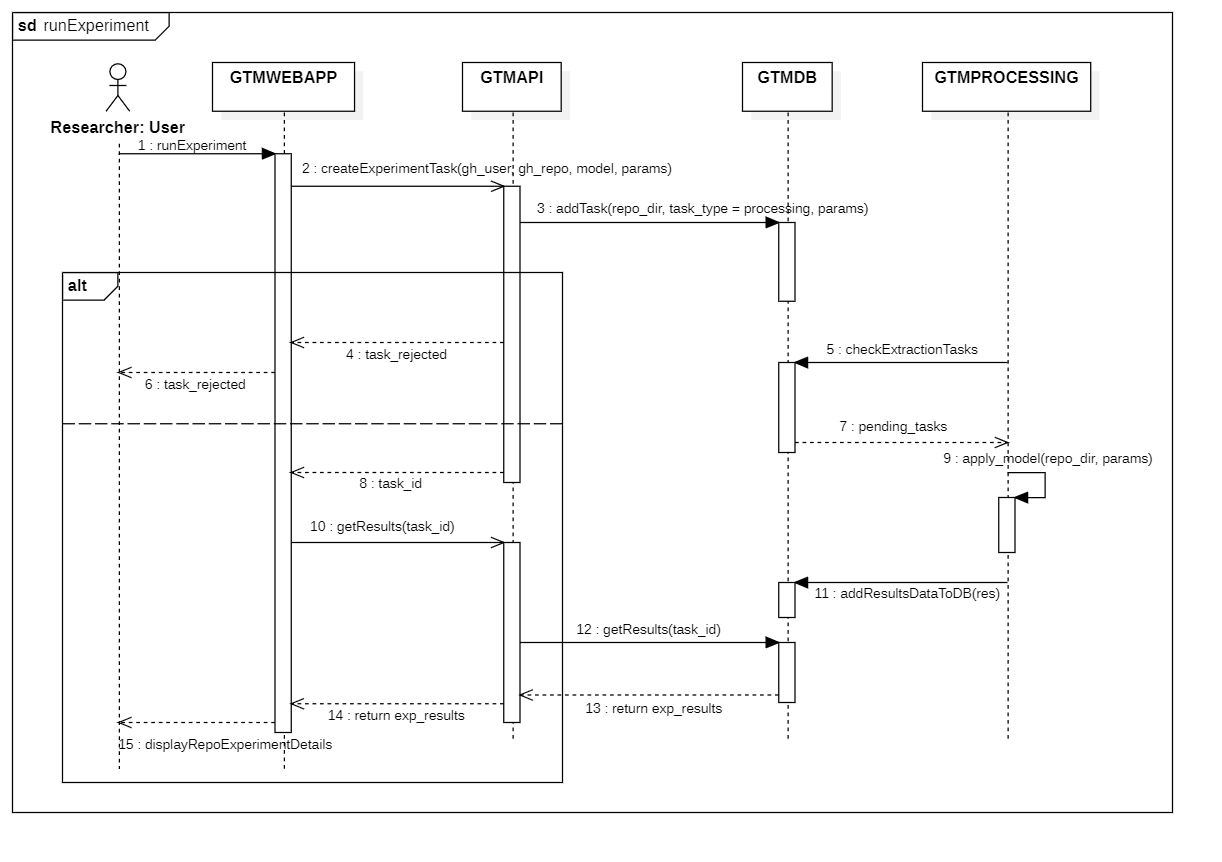
\includegraphics[width=\textwidth]{img/sec_diagram_run_experiment.png}
	\caption{Diagrama de secuencia genérico correspondiente al lanzamiento de un experimento.}
	\label{fig:sec_diagram_run_experiment}
\end{sidewaysfigure}

\clearpage
\section{Diseño arquitectónico} \label{sec:archdesign}

El diseño arquitectónico sobre el que se ha basado la estructura del proceso surge con la finalidad de fraccionar el proceso objetivo en fases más simples que operen de manera independiente. Esta división de los procesos otorga una mayor flexibilidad a la hora de incorporar cambios en alguna de las secciones minimizando los posibles efectos colaterales. La arquitectura que responde a estas características resulta en la utilización de una arquitectura de microservicios como se ha venido mencionando en la memoria.

\subsection{Backend}

El \textit{backend} del proyecto se encuentra conformado por 4 paquetes que desempeñan las funciones requeridas para el cumplimiento con los requisitos funcionales definidos previamente. Estos paquetes son el paquete \textit{gtmcore}, el paquete gtmapi, el paquete \textit{gtmextraction} y el paquete \textit{gtmprocessing}. La estructura interior de los paquetes sigue el esquema reducido de una arquitectura Modelo-Vista-Controlador (MVC) debido a que se enfoca en la estructuración de su código de acuerdo con la generación de una dependencia entre los datos de la aplicación y su lógica. Escalando un nivel se aprecia la dependencia existente entre los paquetes gtmapi, \textit{gtmextraction} y \textit{gtmprocessing} con el servicio \textit{gtmcore}. Este paquete tiene como objetivo dotar a los diversos servicios de aquellas funcionalidades que les permiten interactuar con la información almacenada en la base de datos (véase \autoref{fig:package_diagram}).

\begin{figure}[!ht]
	\centering
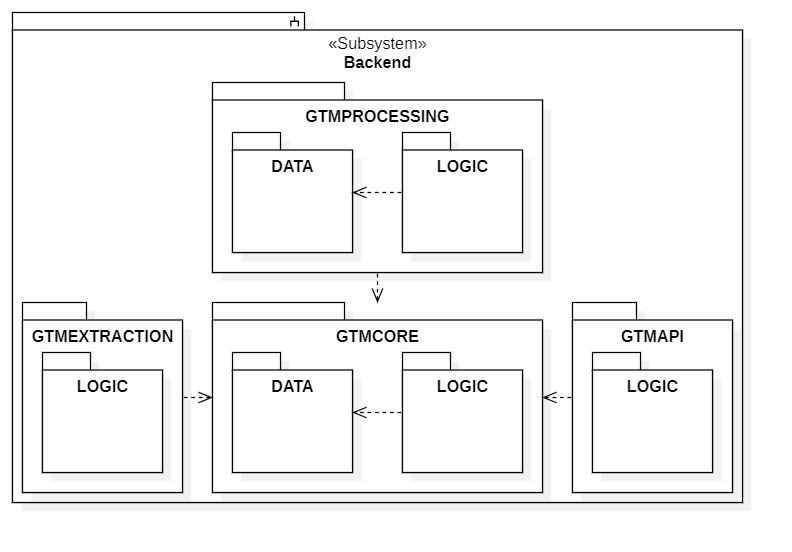
\includegraphics[width=\textwidth]{img/package_diagram.png}
	\caption{Diagrama de paquetes del proyecto.}
	\label{fig:package_diagram}
\end{figure}

Desde el punto de vista de los componentes lógicos que conforman el backend del proyecto, este se divide en cuatro servicios que podemos distinguir en función de su objetivo. El componente \textit{gtmapi} tiene como objetivo generar la interacción de la aplicación con el exterior, sea un usuario u otra aplicación que solicita sus servicios. El componente \textit{gtmextraction} tiene como finalidad establecer la conexión con GitHub y proceder a la extracción de la información de los repositorios. El componente \textit{gtmprocessing} tiene como propósito aplicar los modelos de procesamiento del lenguaje natural sobre la información extraída. Finalmente, el componente de la base de datos actúa como punto de interacción entre los servicios así como de almacén de la información (véase \autoref{fig:component_diagram}).

\begin{figure}[!ht]
	\centering
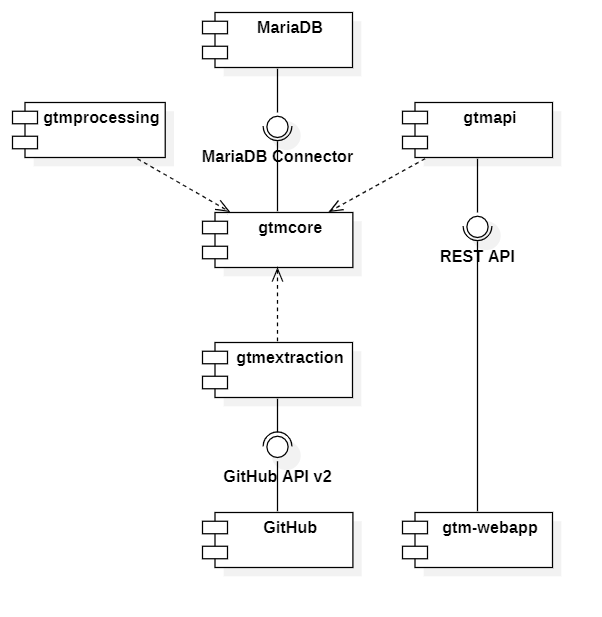
\includegraphics[width=\textwidth]{img/component_diagram.png}
	\caption{Diagrama de componentes del proyecto.}
	\label{fig:component_diagram}
\end{figure}

Acudiendo al diagrama de despliegue se puede observar la distribución física de los componentes de acuerdo con el mecanismo de despliegue que se ha decido utilizar. Los servicios se lanzan de manera aislada por medio de contenedores Docker. Esta distribución permite desplegar desde un mismo equipo varios SO aislados simulando su despliegue en varios equipos diferentes. Según las necesidades de recursos y distribución del proyecto el proyecto podría ser configurado para su despliegue en equipos diferentes siempre y cuando se respeten las vías de comunicación establecidas (véase \autoref{fig:deployment_diagram}).

\begin{figure}[!ht]
	\centering
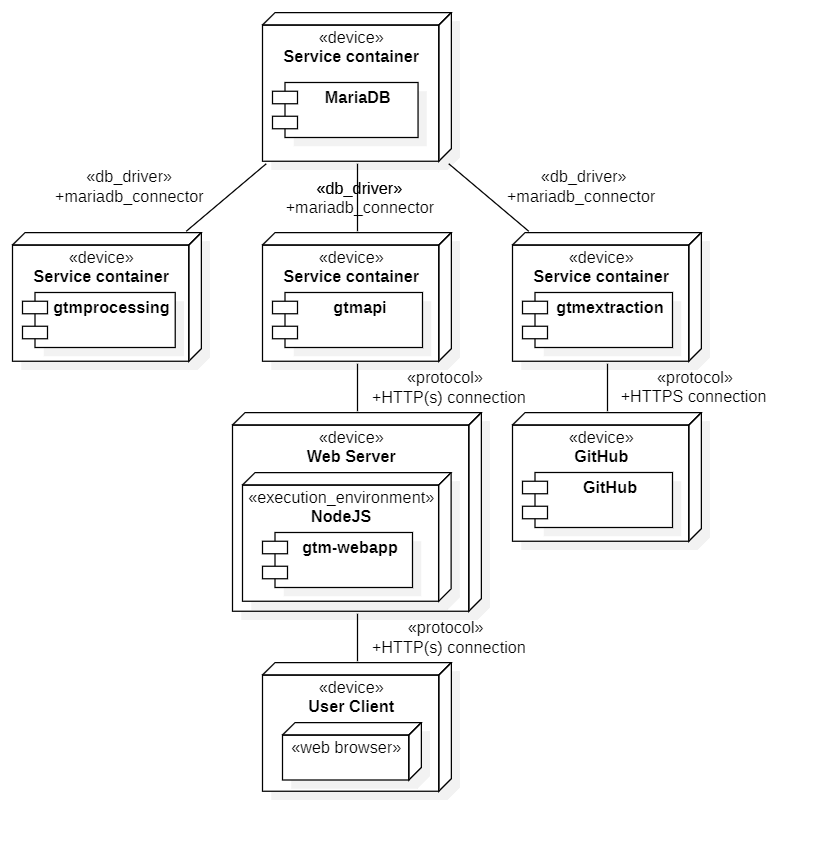
\includegraphics[width=\textwidth]{img/deployment_diagram.png}
	\caption{Diagrama de despliegue que refleja la arquitectura de microservicios implementada en el proyecto.}
	\label{fig:deployment_diagram}
\end{figure}

\subsection{Patrones de Diseño}

\subsubsection{Estrategia}

El patrón estrategia ha sido utilizado en el paquete de \textit{gtmprocessing} con el objetivo de facilitar la ampliación del número de modelos de procesamiento de lenguaje natural implementados en un futuro. El desarrollo se ha producido estableciendo una clase \textit{Project Manager} como Cliente que hace uso de los diferentes modelos (Estrategias) a través de la abstracción Base Model (véase \autoref{fig:class_diagram_processing}).

El uso de la abstracción requiere a sus descendientes de la implementación fundamental de los métodos \texttt{preprocess} y \textit{apply} entre otros. Estos métodos permiten a las subclases personalizar la adaptación necesaria de los datos al formato requerido por las entradas de los modelos. 

\begin{figure}[!ht]
	\centering
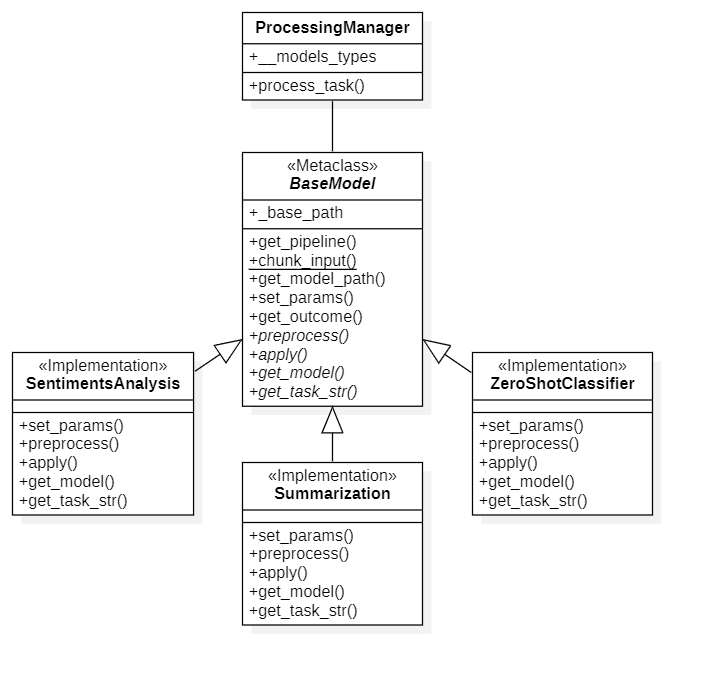
\includegraphics[width=\textwidth]{img/class_diagram_processing.png}
	\caption{Diagrama de clases de la lógica del procesamiento.}
	\label{fig:class_diagram_processing}
\end{figure}

Una particularidad del proceso de desarrollo realizado implica que el patrón estrategia no se ha desarrollado por completo debido a que si así fuese el patrón requeriría que la clase cliente no debería sufrir modificaciones ante la incorporación de nuevos modelos. En este caso, el cliente mantiene un diccionario que asocia una serie de claves con las diferentes implementaciones de los modelos. Pese a esta sutil diferencia, el cliente no requiere de modificaciones en su flujo de actividad principal que puedan alterar el comportamiento de la aplicación y causar puntos de fallo de mayor gravedad.
